\documentclass[a4paper]{article}

%% Language and font encoding
\usepackage[english]{babel}
\usepackage[utf8x]{inputenc}
\usepackage[T1]{fontenc}

%% Sets page size and margins
\usepackage[a4paper,top=3cm,bottom=2cm,left=3cm,right=3cm,marginparwidth=1.75cm]{geometry}

%% Useful packages
\usepackage{amsmath}
\usepackage{graphicx}
\usepackage[colorinlistoftodos]{todonotes}
\usepackage[colorlinks=true, allcolors=blue]{hyperref}
\usepackage[title]{appendix}

% commenting
\usepackage{todonotes}
%\usepackage[draft]{todonotes}   % notes showed

\title{Optical absorption enhanced by an external optical cavity}
\author{Ido Frenkel and Avi Niv}

\begin{document}
\maketitle

%%%% ABSTRACT %%%%
\begin{abstract}
\noindent Optical confinement mechanisms are crucial for enhancing the absorption in high efficiency solar cells. Existing approaches in that regard, as well as conceptual ones, all relay on the cell's active media both for light trapping and charge separation and transport.This places a conflicting requirements on the cell design; on one hand the cell needs to be thick enough to absorb most of the available light while on the other hand it has to be thin enough for allowing substantial amount of the charge carriers reaching the collecting terminals. This conflicts hampers the ability of any existing solar cell, based on any material platform form reaching its full optical and electrical potential simultaneously.Recently external cavities has emerged as a way of light trapping method not being based on the active media of the cell. This has the potential, for the first time, to decouple the optical aspects of the cell design from the electronic ones. In this study We develop a theoretical model for the absorption enhancement of an object that is placed inside and on the surface of an external cavity. We supplement this derivation with and experimental measurements that shows the validity of our approach. The conditions where an external cavity can outperform existing approaches are identified. Specifically it is shown that an Si cell that is as thin as to reach only 50\% absorption, and therefore much better charge transport, may reach more then 90\% absorption by being placed inside a high quality external-cavity.
\end{abstract}

%%%% INTRO %%%%
\section{Introduction}
Solar cells are the converters of light's power radiated from the sun into a more useful form, which is usually electricity. As such, solar cells are required to perform superbly both optically and electronically. These, however, are conflicting requirements; thicker layers form better absorbers, while thinner ones have superior charge transport. Any viable solar cell, based on any material platform, has to negotiate these conflicting requirements to optimize its power. This negotiation is aided by light trapping approaches that allow thinner active layers, with superior charge transport, to maintain high optical absorption. Most notable in that regard are the thous based on randomizing light's rays directions inside the active layer of the cell. Here, the relatively collimated sunlight enters the cell whereupon it is scattered in the front, back, or on both facets of the active layer. This scattering means that some light rays propagates inside the active layer at angles that are beyond the critical angle for total internal reflection (TIR) with respect to the cells facets. Careful evaluation of this situation shows that in this case the average path-length of a ray inside the active layer approaches $4n^2$ times the layer thickness for weakly absorbing media, which will be denoted as the TIR limit henceforth. This phenomenon was first analyzed By Yablonovitch in the framework of statistical ray optics \cite{Yablonovitch82josa} and later also with more advanced techniques \cite{Gee1988, Green2002}. Silicon, for example, is an indirect semiconductor and as such has optical absorption coefficient as low as $1 cm^{-1}$ for at wavelengths just above its $1.1 eV$ bandgap \cite{Si_Prop} \todo{consider replacing this last citation}. This means that if 90\% absorption is required, that an optical path of centimeters is needed. Silicon, however has relatively high refractive index of about $3.6$. Using TIR based trapping, therefore, allows a 50 fold reduction in thickness without scarifying the optical path and the resulting absorption. Indeed, modern solar cells rely on TIR based trapping to achieve exquisite charge transport abilities in active layers of hundred micron or so \cite{GreenIIIgen}. The success of TIR based trapping comes from its simplicity (easy to make) and robustness (broadband and insensitive to the polarization state of light). TIR trapping has its shortcomings as well. For starters, it works best for high refractive indexes materials, like silicon. Other solar cell materials, however, do not posses this advantage. Oxides \cite{Warren2013c}, Organic \cite{chen2018donor}, and even the more recent perovskites \cite{chen2018large}, all have the real part of their refractive index in the range of $2$. The notation of 'real' refractive index brings about the second shortcoming of TIR based approaches. The ray nature of light, which enable this mechanism in the first place, is only valid for low absorbing materials that have negligible imaginary part of their refractive index. One might argue that no trapping is needed if highly absorbing materials are considered, but this is not necessarily true. Highly absorbing materials are often poor transporters of charges; all of the above mentioned can be considered as an example for this observation. In did, a recent study has looked to the merit of solar cell materials in terms of light trapping (termed \emph{photon management}) and charge transport abilities (termed \emph{electron management}) \cite{Polman2016}. There it is shown that with the exception of the high index silicon and Cd:Te, all other materials, even thous with high absorption coefficient like perovskites, has a room for improvement in terms of their light trapping abilities. Discussion along similar lines was also given in \cite{Green2016}.

Naturally, light trapping methods aiming at surpassing TIR-based approaches have emerged. These mainly rely on the ability to confine electromagnetic radiation at the immediate vicinity of subwavelength structures using plasmonic or photonic effects \cite{Atwater2010a, Polman2012a}. Despite the considerable progress that was achieved so far \cite{Pala2009, Massiot2012}, none of the proposed approaches rivals TIR when it comes to utility and cost-effectiveness. The reason these new approaches fall short has a lot to do with their reliance on wave-optics, which is inherently sensitive to the wavelength, illumination-direction, and polarization of light. Solar cells, on the contrary, feed on broadband, often omnidirectional, and unpolarized natural-light - properties that are best handled using ray-optics.  

Recently, a new approach emerged that has the potential for optical-ray-based trapping even for highly absorbing ultra thin material where traditional TIR-based approaches has failed. In this approach the solar cell is placed inside an external optical device whose sole purpose is light trapping. This approach first emerged as a means of increasing the open circuit voltage in photovoltaics with high external luminescence efficiency \cite{Braun2013_external_recycling}, but it potential for enhancing the absorption and therefore the current was soon appreciated \cite{Weinstein2014a,Weinstein2015b,Niv2016a}, as well as its ability to recover lost reflection losses \cite{VanDijk2016a}. External cavities has, however, the potential for a much deeper paradigm shift in solar cell design as they allow, for the first time, to decouple the cell's electronic and optical functionalists. This fact liberates the cell design to pursue optimal charge separation and transport, while leaving the task of recovering the lost optical absorption to the external optical device \cite{VanDijk2016a}. 
\par % what have we done
In this paper we use flux balancing approach to derive close-form expressions for the absorption enhancement of a cell placed inside, or against the wall of, an external cavity. The model considers the area of the cavity, the area of its port, its inner surface reflectively, and the area and absorption of the target cell (denoted henceforth as target). further, it is assumes that complete randomization of the light rays inside the cavity prevail. As we shall later show by comparison with ray optics simulations and experimental measurements, this single assumption places the most severe limitations on the proposed model.
% what have we found
\todo{update reconstructed absorption (marked ???)}
The model shows that a realistic model of external cavity is able to reconstruct ???\% absorption for a cell (target) with native absorption of 50\%.
\par % manuscript layout
The paper is organized as follow:
    % 1. theoretical derivation
    First, close-form expressions are derived based on balancing the incoming, outgoing, and absorbed optical fluxes of the cavity. The resulting expressions are then used to derive the expected cavity performance for different system parameters such as port are, and target absorptivity.
    % 2. simulation and its connection with the theory
    \todo{this is so far a fictional paragraph}
    Next a cavity is simulated using ray optics model and the results are matched against the analytic model. It shows that the theoretical model is most jeopardized by optical-filed inhomogeneity caused be excess of cavity losses.
    % 3. experiment and its connection to theory and simulation
    A real-world evaluation of the model is gotten by constructing a cavity using a $15cm$ diameter spectroscopic integrating sphere. The measured results are in good agreement with simulation. Accordingly, the range of validity of the closed-form expressions is reinforced.
    % 4. Summery and conclusions
    Finally, the main findings of our investigation are summed-up and some conclusions are drawn.
\todo{find out where to speak of analysis models}

\par Various forms of flux balancing approaches have been used in the past to analyze the performance of TIR light trapping. In his seminal paper \emp{Statistical ray optics} Yablonovitch has balance the incoming and outgoing fluxes to derive his famous $4n^2$ limit. This is, however, considers only week-absorbing materials \cite{Yablonovitch1982} . An improvement to the model was proposed by Gee \cite{Gee1988}, and later by Green \cite{Green2002}, in the form of two-flux model that can account for the actual absorption along the path length of a ray.
% talk about the planar layered structure and the four-flux and BDSF formalism's, as well as their shortcomings.
 
\listoftodos\bigskip
\section{The cavity flux balancing optics}

% introducing the system
\noindent This paper studies the consequences of placing a solar cell inside an external cavity. We start with analyzing the potential for broadband-light absorption enhancement for a piece of material placed inside a cavity. Figure \ref{fig:sys} gives a schematic view of the system under consideration: Light that falls on the concentrator, depicted here as a lens, is focused onto the entrance port of the cavity. The cavity is a spherical reflecto-scattering shell filled with a transparent media with a (real) refractive index $n$. Light that enters the port is randomized by multiple reflection off the cavity wall. Ideally, the chances that a ray might find its way out is simply the port to wall area fraction. The effect of cavity losses and target absorption on this merit is the main objective of this paper.
% flux balancing
\par

\begin{figure}
\centering
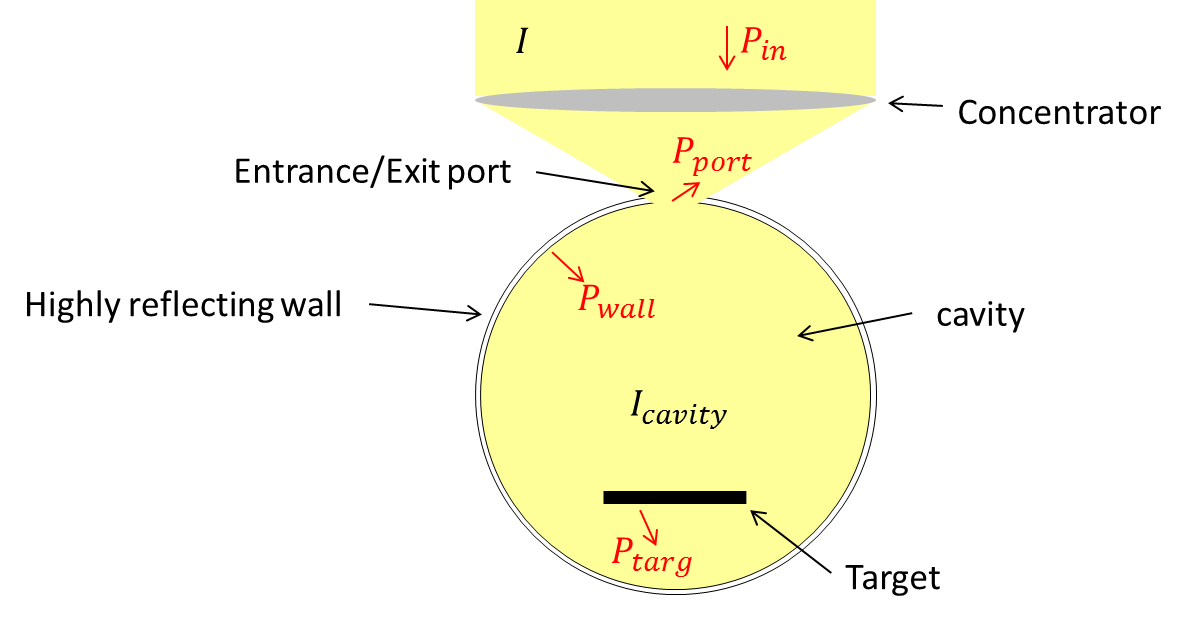
\includegraphics[width=0.8\textwidth]{figures/cav3.png}
\caption{Schematic view of the cavity, target, and concentrator. Fluxes are denoted with red arrows.}
\label{fig:sys}
\end{figure}

%In the following we derive the concentration factor of light inside a cavity. The derivation is based on the assumption that rays are a valid description of light for this case, i.e. the cavity and all of its ports are many wavelength in size. Another assumption is that the light-rays are randomized in their directions due to multiple reflections from the Lambertian (perfectly scattering) cavity walls. Based on the apparatus from Fig. \ref{fig:system}, $P_{in} (W)$, the power entering the cavity is:

\subsection{flux balancing}
In the following we develop what should be the light’s intensity on the target for a given cavity parameters of interest such as the geometrical concentration, cavity area, port size, and cavity wall absorptivity. The calculations are based on three assumptions: First we assume that any geometrical dimension of the system, cavity + concentrator, is much larger then the typical optical wavelength involved such that ray optics is valid description of the light. Second, we assume that the light inside the cavity is completely randomized due to multiple reflections of the cavity walls, and third we assume that the external light source is completely coherent. The first allow us use flux-balancing method to derive the expected performance of the cavity.The second allows to neglect the specular (collimated) flux inside the cavity, thus considerably simplifying the analysis. The third allow a simple account of the incoming power. Out of the three, the second is the fragile one. As we shall see later, violation of the second assumption in the form of inhomogeneous intensity inside the cavity leads to some deviation of the measured values relative to the expected ones. Correction factors are the incorporated that brings the predicted and measured values to an excellent agreement.



\section{The cavity optics}\label{sec2}

\subsection{The cavity concentration factor}


\begin{equation}\label{eq1}
P_{in}=IA_{con},
\end{equation}

\noindent where $I (W/m^2)$ is the intensity, taken as one sun in our case, and $A_{con}$ is the collecting area of the concentrator. Since a cavity is a passive device the entering power has to be balance by the power leaving the cavity as heat or radiation:

\begin{equation}\label{eq2}
P_{in}=P_{wall}+P_{port}+\sum_{i} P_{targ},
\end{equation}

\noindent where $P_{wall}$ is the power lost to the cavity-wall absorption, $P_{port}$ is the power that escapes through the entrance port, and $P_{targ}$ is the power absorbed by the target material, which designates the solar cell or any other system of interest. The index $i$ accounts for the situation where there are multiple targets inside the cavity. Assuming the intensity inside the cavity $I_{cavity}$ is homogeneous and that the target is centered inside the cavity (the case of placing the target against the wall would be discussed in section \ref{sec3}, the right side of equation \ref{eq2} can be expressed as:

\begin{equation}\label{eq3}
P_{wall}=I_{cavity}\alpha_{wall}(A_{cavity}-A_{port}),
\end{equation}

\begin{equation}\label{eq4}
P_{port}=I_{cavity}\alpha_{port}A_{port},
\end{equation}

\begin{equation}\label{eq5}
P_{targ}=I_{cavity}\alpha_{targ}A_{targ},
\end{equation}

\noindent where $\alpha_{wall}$ is the absorptance of the cavity wall, $A_{cavity}$ is the surface area of the cavity – ports included, $\alpha_{port}$ is the entrance port power transmission, $A_{port}$ is the port area, $\alpha_{targ}$ is the target absorptance and $A_{targ}$ is the target area. 
Combining equations \ref{eq1}-\ref{eq5} gives:

\begin{equation}\label{eq6}
IA_{con}=I_{cavity}\Big[\alpha_{wall}(A_{cavity}-A_{port})+\alpha_{port}A_{port}+\sum_{i}\alpha_{targ}A_{targ}\Big],
\end{equation}
\noindent and upon rearrangement the concentration factor emerges:

\begin{equation}\label{eq7}
C_{tot} \equiv \frac{I_{cavity}}{I} = \frac{A_{con}}{\alpha_{wall}(A_{cavity}-A_{port})+\alpha_{port}A_{port} + \sum_{i}\alpha_{targ}A_{targ}},
\end{equation}

\noindent Which can also be expressed as:

\begin{equation}\label{eq8}
C_{tot} = \frac{f_{con}}{\alpha_{wall}(1-f_{port}) + \alpha_{port}f_{port} + \sum_{i}\alpha_{trag}f_{targ}},
\end{equation}

\noindent Where the following are defined: $f_{con}=A_{con}/A_{cavity}$, $f_{port}=A_{port}/A_{cavity}$, $f_{targ}=A_{targ}/A_{cavity}$. Equation \ref{eq8} express $C_{tot}$ as the product of two factors: One, $f_{con}$, is purely geometrical while the  second, $C_{cavity}$, expresses the enhancement of lights intensity inside the cavity relative to the intensity just outside its port. The later is termed the \emph{cavity concentration factor} henceforth. It is important to note that $f_{con}$ is anything between zero and infinity and the following inequality holds: $\frac{1}{\alpha_{port}f_{port}}\geq C_{cavity}$, where equality emerges if the cavity wall is a perfect scattering reflector and no target is placed inside. On the contrary, minimal $C_{cavity}$ is gotten for completely absorptive wall and target. Figure \ref{fig:concentration_factor} shows $C_{cavity}$ as a function of different cavity parameters. Figures \ref{fig:concentration_factor}(A) shows $C_{cavity}$ as a function of $f_{port}$ for different values of $\alpha_{wall}$. For high values of $f_{port}$, $C_{cavity}$ is minimal and the effect of $\alpha_{wall}$ on $C_{cavity}$ is minimal. Figures \ref{fig:concentration_factor}(B) shows $C_{cavity}$ as a function of $f_{targ}$ for different values of $\alpha_{wall}$. Here, the trends are similar to those of Fig. \ref{fig:concentration_factor} but the values of $C_{cavity}$ become minimal already around $f_{targ}=0.2$. Figure \ref{fig:concentration_factor}(C) show $C_{cavity}$ as a function of $f_{port}$ for different values of $\alpha_{targ}$. Again, we see here the same trend, where for values of $f_{port}>0.2$ the effect of $\alpha_{targ}$ on $C_{cavity}$ is minimal. We also see that $C_{cavity}$ is very sensitive to small changes of $\alpha_{targ}$ at low values of $f_{port}$. Figure \ref{fig:concentration_factor}(D) show $C_{cavity}$ as a function of $f_{targ}$ for different values of $\alpha_{targ}$. Here, we see a slightly different trend, where although there is a reduction of $C_{cavity}$ when $f_{targ}$ increase, it is still maintain different values for different values of $\alpha_{targ}$. 

\begin{figure}
\centering
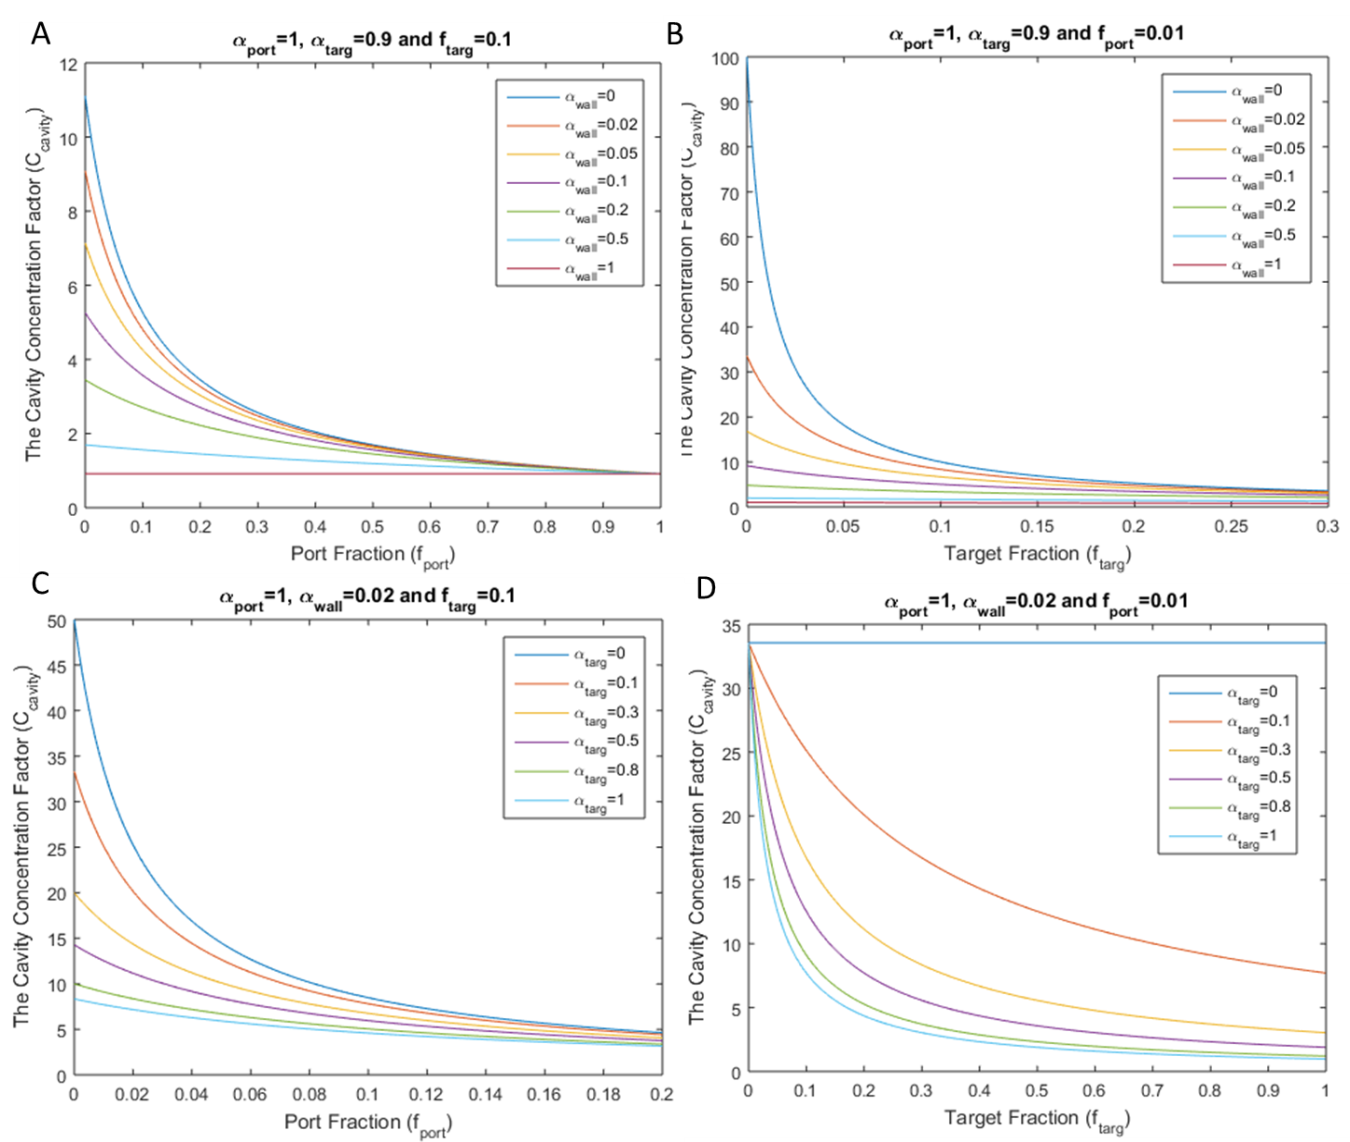
\includegraphics[width=1\textwidth]{figures/concentration_vs_parameters.png}
\caption{(A) The cavity concentration factor $C_{cavity}$ as a function of the port fraction $f_{port}$ for different $\alpha_{wall}$, where  $\alpha_{port}=1$, $\alpha_{targ}=0.9$ and $f_{targ}=0.1$. (B) The cavity concentration factor $C_{cavity}$ as a function of the target fraction $f_{targ}$ for different $\alpha_{wall}$, where $\alpha_{port}=1$, $\alpha_{targ}=0.9$ and $f_{port}=0.01$. (C) The cavity concentration factor $C_{cavity}$ as a function of the port fraction $f_{port}$ for different $\alpha_{targ}$, where $\alpha_{port}=1$, $\alpha_{wall}=0.02$ and $f_{targ}=0.1$. (D) The cavity concentration factor $C_{cavity}$ as a function of the target fraction $f_{targ}$ for different $\alpha_{targ}$, where $\alpha_{port}=1$, $\alpha_{wall}=0.02$ and $f_{port}=0.01$.}
\label{fig:concentration_factor}
\end{figure}

\subsection{Concentration factor considerations}
\subsection{Enhancement of absorption}
\subsection{Enhancement of the target absorption compared to TIR}
\subsection{General case: a cavity filled by a material}
\section{Special case: the target is on the cavity wall}\label{sec3}
\section{Example: a target inside a cavity vs a target outside the cavity}
\section{A solar cell as our target}
\subsection{The effect of concentration}
\subsection{The effect of photon recycling}
\section{Experimental investigation of the cavity performance}
The cavity measurement was made in order to verify our suggested model using an integrating sphere (Gigahertz-Optik UPB-150-ARTA). Figure \ref{fig:setup} shows the schematics of the measurement system. Light from a fiber illuminator (FI, OSL2 Fiber illuminator)  is concentrated by an objective lens (OL, Newport objective M-10X) into one of the integrating spheres port, the light propagate inside the cavity by reflecting of its highly reflective walls. A power meter (PM, X1-1 Optometer) is placed at the bottom of the sphere and measures the intensity inside the cavity. a baffle was placed in front (or next to) the detector, to avoid measuring direct radiation which could affect the fit to the model. The cavity had 3 types of port openings (3mm,1cm, and 3cm diameters) and a top opening (4.5cm diameter) that was also used for the target holder. Since the measurement is a relative measurement between the incoming intensity to the cavity vs the intensity inside the cavity (will be discussed later), before each set of measurements, a direct measurement of the incoming light was performed. The power meter of the integrating sphere was placed directly in front of the objective and a measurement was taken. The cavity inner diameter was taken to be 14.5cm.

\begin{figure}
\centering
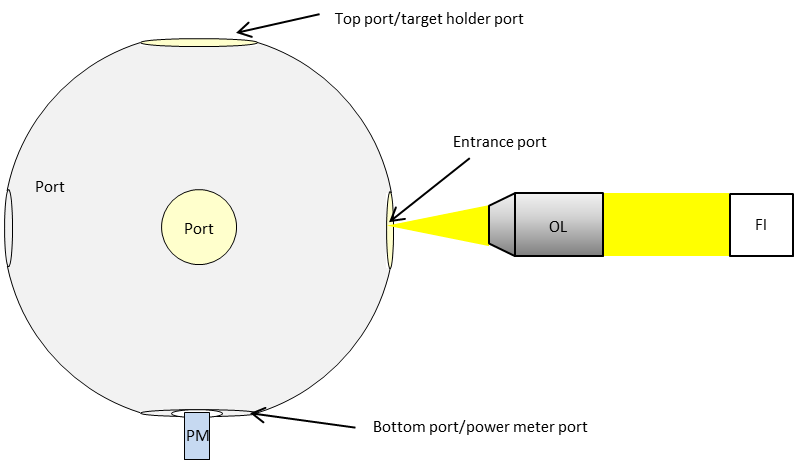
\includegraphics[width=1\textwidth]{figures/cavity_measurement_system.png}
\caption{\textbf{Schematics of the measurement system.} Light from a fiber illuminator (FI, OSL2 Fiber illuminator)  is concentrated by an objective lens (OL, Newport objective M-10X) into one of the integrating spheres port, the light propagate inside the cavity by reflecting of its highly reflective walls. A power meter (PM, X1-1 Optometer) is placed at the bottom of the sphere and measures the intensity inside the cavity. A baffle was placed in front (or next to) the detector, to avoid measuring direct radiation which could affect the fit to the model. The cavity had 3 types of port openings (3mm,1cm, and 3cm diameters) and a top opening (4.5cm diameter ) that was also used for the target holder.}
\label{fig:setup}
\end{figure}

measurements that have been preform examined the intensity inside the cavity vs the opening port size for an empty cavity and for different sizes of a highly absorbing material (BKF12 Thorlabs) that was placed inside the cavity. Since this measurement is a relative measurement, using equations \ref{eq1} and \ref{eq6} (from the theoretical part) the relative measured power between the measured power $P_{PM}$ and the input power. $P_{in}$ was taken to be:

\begin{equation}\label{eq_measurement}
P_{rel}=\frac{P_{PM}}{P_{in}}=\frac{Df_{SC} \alpha_{PM}}{D\alpha_{wall} (1-f_{port}-f_{PM})+\alpha_{port} f_{port}+\alpha_{PM} f_{PM}+T\alpha_{targ} f_{targ}+\alpha_{h} f_{h}} ,
\end{equation}

In our case $\sum_{i}\alpha_{targ}A_{targ}$ from equation \ref{eq_measurement} was taken to be: $\sum_{i}\alpha_{targ}A_{targ}=\alpha_{PM} A_{PM}+\alpha_{targ} A_{targ}+\alpha_{h} A_{h}$ Where the subscripts $PM$, $targ$ and $h$ correspond to the power meter total area, the target and the target holder respectively. The subscript $SC$ correspond to the semiconductor area of the semiconductor in the power meter. $D$ and $T$ are constants representing the correction of the fit due to inhomogeneous radiation inside the cavity (will be further discuss later). The measurement was performed by opening the ports of the sphere. The total amount of possible combination of port openings was 72, but since some of the combinations had the same opening size but was located at different ports, the amount of combinations was reduced to 40. Figure \ref{fig:72vs40} shows the relative light intensity vs the port fraction for the 72 combination measurement (blue) and the 40 combination measurement (black). We can clearly see that there is not much different between the configurations and thus the 40 combination configuration was chosen for the measurements. The order of the ports that was opened was repeated for all measurement to avoid additional deviations (discussed at appendix).

\begin{figure}
\centering
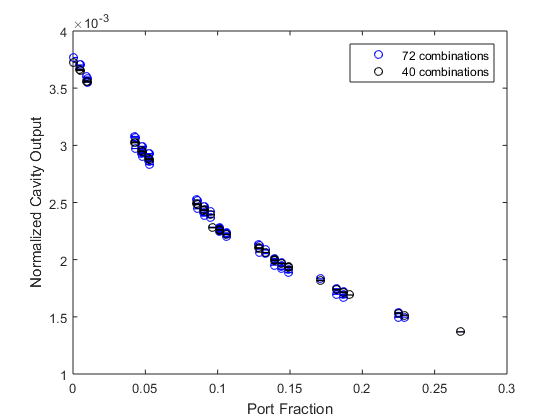
\includegraphics[width=0.8\textwidth]{figures/72vs40.png}
\caption{\textbf{72 configurations of port openings vs 40 configurations of port opening.} The normalized intensity inside the cavity was measured vs the port fractions in two different configurations, 72 combinations of the port opening where several port fraction sizes repeated and 40 combinations of the port opening where no port fraction size repeated.}
\label{fig:72vs40}
\end{figure}

During the measurements it occurred that the light interacting with the detector might not be homogeneous enough and/or that the baffle was not preventing some direct light from reaching the power meter. This can significantly affect the results fit to the suggested model. Figure \ref{fig:baffles_full}(A) shows the relative light intensity vs the port fraction for 2 different baffle types in 3 different configurations: 1) parallel baffle 2) side baffle facing the light entrance port and 3) side baffle facing opposite to the light entrance port (shown in \ref{fig:baffles_full}(B)). Figure \ref{fig:baffles_full} also shows another examination where the third configuration measurement was repeated for different incoming light intensity. We can see that there is a different result just by changing the baffle configuration where the baffle facing opposing to the light entrance port shows the lowest values. This means that the detector does not get fully homogenized radiation and this will have to be taken into consideration. In addition, as expected, we can see that changing the incoming light intensity, does not change the results.

\begin{figure}
\centering
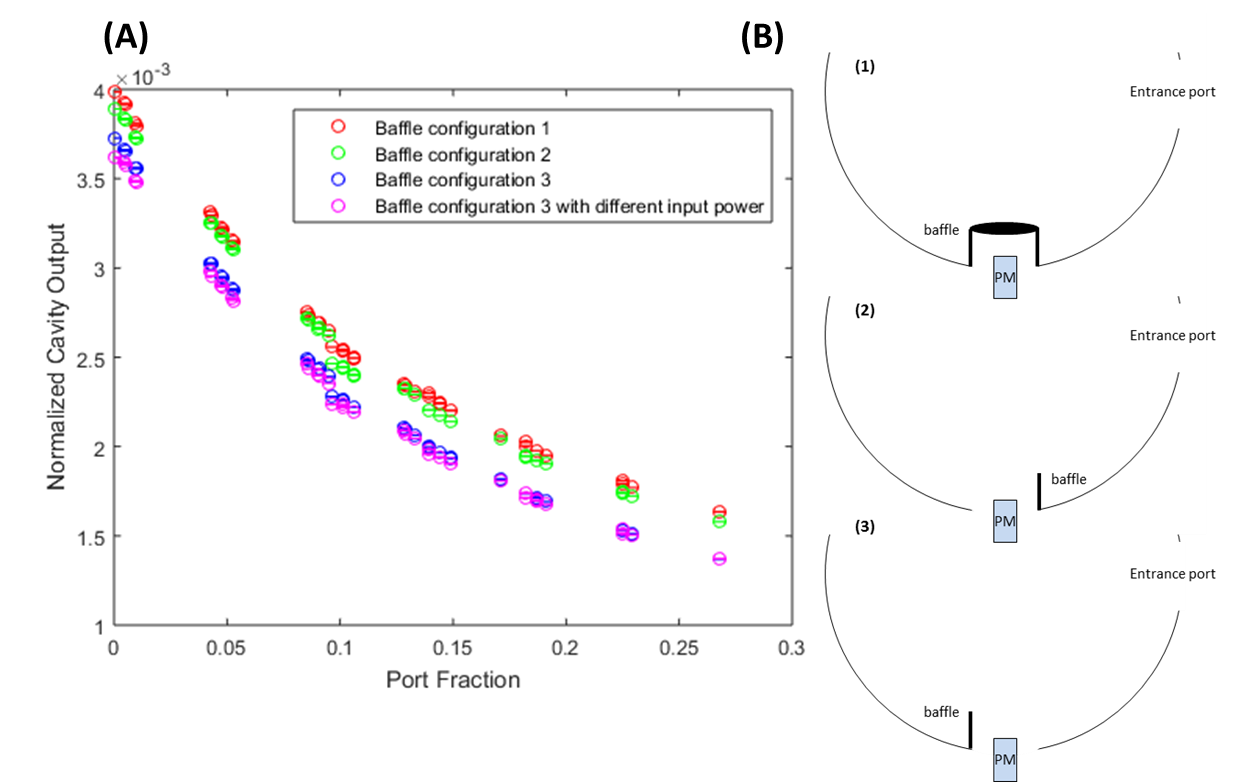
\includegraphics[width=0.8\textwidth]{figures/baffles_full.png}
\caption{\textbf{The normalized cavity output vs the port fraction for different baffle configurations.} (A) The relative light intensity vs the port fraction for 2 different baffle types in 3 different configurations: (B1, red circles) parallel baffle (B2, green circles) side baffle facing the light entrance port and (B3, blue circles) side baffle facing opposite to the light entrance port. The magenta circles show another examination where the third configuration measurement was repeated for different incoming light intensity.}
\label{fig:baffles_full}
\end{figure}

Figure \ref{fig:target_size} shows the relative light intensity vs the port fraction for different target sizes: no target (blue), only target holder (green), $f_{targ}=0.00835$ (red), $f_{targ}=0.0174$ (magenta), $f_{targ}=0.0356$ (cyan), $f_{targ}=0.0477$ (black) and $f_{targ}=0.0719$ (yellow). The fit parameters were as follows: $\alpha_{wall}=0.063$, $\alpha_{port}=1$, $\alpha_{targ}=0.95$, $\alpha_{h}=0.39$, $\alpha_{PM}=1$, $f_{SC}=0.000242$,  $f_{PM}=0.001712$, $f_{h}=0.038$. We can see that as expected, the bigger the target is, the lower the measure relative intensity inside the cavity. The target was oriented parallel to the light entrance port so it will create minimal shade on the opposite wall to the light entrance port. This was chosen in order to avoid direct light absorption and reflection by the target as much as possible. It should be noted that since some of the targets was not fully straight and had some small deformations due to the material properties which created some shade on the opposite wall to the light entrance port. This means that some of the direct light was absorbed and reflected by it and had to be considered as well at the fit model in the form of the factor T. T can vary from 1, where there is no shade by the target, to infinity, where the target fully absorb the incoming direct radiation. An increase of T also lead to a reduction of D since less radiation propagate inside the cavity and reach the power meter. It is possible that bigger baffles may remove the need of D. when the cavity is empty or even with the target holder inside $D=2.1$ (because the target holder does not shade the direct radiation path) but, when $T=1.8;1.9;1.95;1.75$ it reduces to $D=2;1.9;1.95;2$ respectively. Moreover, when we intentionally increase the shade created by the target, as shown in Fig \ref{fig:target_size}, where $f_{targ}=0.0477$ but oriented 10 degrees from the origin measurement (black triangles), we can see a reduction of the intensity and thus increase the value of $T$ to $T=2.3$ and a reduction in $D$ to $D=1.9$.

\begin{figure}
\centering
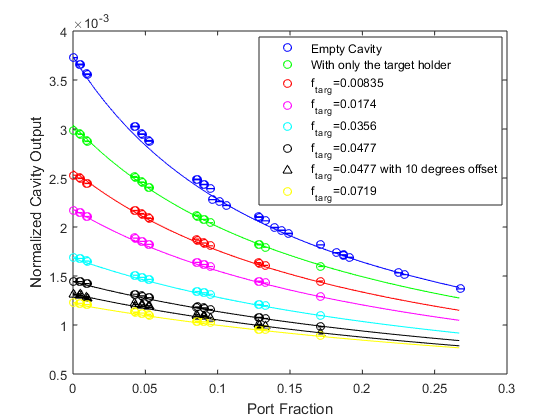
\includegraphics[width=0.8\textwidth]{figures/target.png}
\caption{\textbf{The normalized cavity output vs the port fraction for different target sizes.} The relative light intensity vs the port fraction for different target sizes: no target (blue), only target holder (green), $f_{targ}=0.00835$ (red), $f_{targ}=0.0174$ (magenta), $f_{targ}=0.0356$ (cyan), $f_{targ}=0.0477$ (black) and $f_{targ}=0.0719$ (yellow). The fit parameters were as follows: $\alpha_{wall}=0.063$, $\alpha_{port}=1$, $\alpha_{targ}=0.95$, $\alpha_{h}=0.39$, $\alpha_{PM}=1$, $f_{SC}=0.000242$,  $f_{PM}=0.001712$, $f_{h}=0.038$.}
\label{fig:target_size}
\end{figure}

\section{Summary and conclusions}

\begin{appendices}
\section*{Appendix 1: Estimation of the measurement error}
In order to estimate the full error of relative power $P_{rel}$, several errors were taken into consideration; the standard deviation of the measured power inside the cavity $P_{PM}$, the variations of the background light $P_{background}$ between measurements and the standard deviation of input power $P_{in}$. The error was taken to be:
\begin{equation}\label{eq_error}
\Delta P_{rel}=\frac{\Delta P_{PM}}{P_{in}}+\frac{\Delta P_{background}}{P_{in}}+\frac{\Delta P_{in}(P_{PM}+P_{background})}{P_{in}^{2}},
\end{equation}

\noindent Where $\Delta$ represent the error

\section*{Appendix 2: The measurement sequence}
Figure \ref{fig:cavity_top_view} shows schematics of the cavity from the top. The sequence of opening was as follows:  for every type of port opening, the first port that was open was the port located 90 degrees of the light entrance port, marked as 1 on Fig \ref{fig:cavity_top_view}. The second one opened was port 2 and the third was port 3. If a different type of port was placed, it was first placed at port 1 and a second type was placed at port 2 and so on. The port that was in front of the light opening port was always kept close to prevent direct light from escaping the cavity. Measurements were taken over a period of roughly 45 seconds to reduce noise error (30 measurements in each cycle). Background measurements were taken for each configuration of the system to reduce the error. 

\begin{figure}
\centering
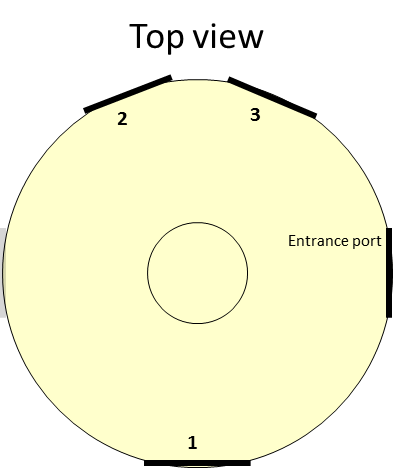
\includegraphics[width=0.5\textwidth]{figures/measurement_sequence.png}
\caption{\textbf{Schematic top view of the cavity.}}
\label{fig:cavity_top_view}
\end{figure}

\end{appendices}

%\bibliographystyle{plain}
\bibliographystyle{unsrt}
\bibliography{mendeley_an,url_lib}

\end{document}